\documentclass[a4paper, twoside, 11pt]{book}

% ============
% = PACKAGES =
% ============
\usepackage[utf8]{inputenc}
\usepackage[Lenny]{fncychap} % chapter customized typo
\usepackage[vscale=0.75,
            hscale=0.75, 
            hmarginratio=5:4, 
            vmarginratio=1:1, 
            marginparsep=5pt, 
            marginparwidth=2cm, 
            headheight=15pt]{geometry} % layout
\usepackage{graphicx} % graphics
\usepackage{amsmath, amssymb} % math
\usepackage{algorithm, algorithmic} %algorithms
\usepackage[tight]{subfigure} % subfigures
\usepackage{xspace} % space at end of macros
\usepackage{fancyhdr} % head of chapters (using lhead)
\usepackage{tabularx, caption}
\usepackage[square, sort&compress, numbers]{natbib}
\usepackage{pdfpages} % to insert a pdf right into the thesis
\usepackage[pagebackref=true, final, colorlinks=true]{hyperref} % hyperlinks
\usepackage{todonotes}

\graphicspath{{./FIGS/}{./PRIMITIVES/}} % Specifies the directory where pictures are stored

% ================
% = NEW COMMANDS =
% ================
\newcommand{\ra}[1]{\renewcommand{\arraystretch}{#1}}

\begin{document}

\listoftodos

\cleardoublepage

%!TEX root = ../../adrien_gomar_phd.tex

\chapter*{Abstract}
\thispagestyle{empty}

TEMP

\chapter*{Résumé}
\thispagestyle{empty}

TEMP


\tableofcontents
\listoffigures

\input{./CHAPTERS/nomenclature}

\mainmatter

%!TEX root = ../main.tex

fil rouge:

"there is always a need for developing efficent methods for applications 
to blade designs. In a design cycle, a large number of flow solutions
are sought to interact iterativeley or concurrently with various options
opportunities and constraints from other disciplines"

% # Flow around contra-rotating open rotors: general information
%     * Background
%     * Aerodynamic of an isolated propeller
%     * Aerodynamic of a contra-rotating open rotor
%     * A few words on aeroelasticity
%         - experimental aeroelasticity
%         - numerical aeroelasticity
% 
% # Generalities
%     * equation that I solve
%     * elsA
%     * ALE / aeroelasticity presentation
%!TEX root = ../../main.tex
\chapter{Generalities}
\label{generalities}

\lhead{Chapitre ??. \emph{Generalities}}

\section{Equation solved} % (fold)
\label{sec:equation_solved}

The Unsteady Reynolds-Averaged Navier-Stokes (U-RANS) equations in
integral form are given by
\begin{equation}
   \int_\Omega \frac{\partial W}{\partial t} dV + \oint_{\partial
     \Omega} \overrightarrow{F} \cdot \overrightarrow{N} ds = 0,
   \label{eq:intNS}
\end{equation} 
where $\overrightarrow{F}$~is the flux across $\partial \Omega$ and
$W$~is the vector of the conservative unknowns (conservative variables
and turbulent variables).  Assuming $\Omega$ is a
control volume, the semi-discrete finite-volume form of the
U-RANS equations is obtained from Eq.~\eqref{eq:intNS}:
\begin{equation}
   \frac{d}{dt} \left(V  \overline{W}\right) + R \left( \overline{W}
   \right) = 0,
   \label{eq:semiDiscNS}
\end{equation} 
with $V$~the volume of the cell~$\Omega$, $R$~the residual resulting
from the discretization of the fluxes and the source terms (including
the turbulent equations), and $\overline{W}$ the mean of the
unknowns over the control volume.  In the following, the over line
symbol~$\overline{\cdot}$ is dropped out for clarity.

% section equation_solved (end)

% 
% # Harmonic balance methods
%     * state of the art
%         - Numeca
%         - Duke
%         - He
%     * mono-frequential
%         - theory
%         - advantages
%         - applications that can be treated
%!TEX root = ../main.tex
\chapter{Harmonic balance methods} % (fold)
\label{cha:harmonic_balance_methods}

The harmonic balance methods are now presented. 
We distinguish two cases: the case where the 
variables are assumed to be periodic in time and the one
where the variables are almost-periodic. This last can be defined as 
a variable that is composed of several frequencies which 
are not harmonically related. This is for example the case of 
$a=\pi$ and $b=1$. There is no integer $k$ that satisfies:
\begin{equation}
    a = k b.
\end{equation}
This leads to two methods, the time spectral method and the
harmonic balance method respectively.

In the following, we will consider the
the Unsteady Reynolds-Averaged Navier-Stokes (U-RANS) equations written in
integral form
\begin{equation}
   \int_\Omega \frac{\partial W}{\partial t} dV + \oint_{\partial
     \Omega} \overrightarrow{F} \cdot \overrightarrow{N} ds = 0,
   \label{eq:intNS}
\end{equation} 
where $\overrightarrow{F}$~is the flux across $\partial \Omega$ and
$W$~is the vector of the conservative unknowns (conservative variables
and turbulent variables).  Assuming $\Omega$ is a
control volume, the semi-discrete finite-volume form of the
U-RANS equations is obtained from Eq.~\eqref{eq:intNS}:
\begin{equation}
   \frac{d}{dt} \left(V  \overline{W}\right) + R \left( \overline{W}
   \right) = 0,
   \label{eq:semiDiscNS}
\end{equation} 
with $V$~the volume of the cell~$\Omega$, $R$~the residual resulting
from the discretization of the fluxes and the source terms (including
the turbulent equations), and $\overline{W}$ the mean of the
unknowns over the control volume.  In the following, the over line
symbol~$\overline{\cdot}$ is dropped out for clarity.

\section{Periodic flows} % (fold)
\label{sec:periodic_flows}

\subsection{Theory}

If the mean flow variables $W$~are periodic in time of period $T =
2\pi/\omega$, so are the residuals $R(W)$ and the Fourier series of
Eq.~\eqref{eq:semiDiscNS} is
\begin{equation}
  \label{eq:seriefour}
  \sum_{k=-\infty}^\infty \left(ik\omega
    V\widehat{W}_k+\widehat{R}_k\right)e^{ik\omega t}=0,
\end{equation}
where $\widehat{W}_k$ and $\widehat{R}_k$ are the Fourier coefficients
of $W$ and $R$ corresponding to the mode~$k$:
\begin{equation}
   W(t) = \sum_{k=-\infty}^{\infty} \widehat{W}_k e^{i k\omega t},\quad
   R(t) = \sum_{k=-\infty}^{\infty} \widehat{R}_k e^{i k\omega t}.
   \label{eq:fourierWsf}
\end{equation}
The complex exponential family forming an orthogonal basis, the only
way for Eq.~\eqref{eq:seriefour} to be true is that the weight of
every mode $k$ is zero, which leads to an infinite number of steady
equations in the frequency domain:
\begin{equation}
  \label{eq:orthodelim}
  ik\omega V\widehat{W}_k+\widehat{R}_k=0, \quad \quad \forall k \in
  \mathbb{Z}.
\end{equation}
McMullen~\emph{et al.}~\cite{McMullen2001,McMullen2002,McMullen2006}
solve a subset of these equations up to mode~$N$, $-N\leq k\leq N$,
yielding the Non-Linear Frequency Domain (NLFD) method.

The principle of the time-domain Harmonic Balance
approach~\cite{Hall2002}, sometimes referred to as Time Spectral
Method (TSM)~\cite{Gopinath2005, Sicot2008}, is to use an Inverse
Discrete Fourier Transform (IDFT) to cast back this subset of $2N+1$
frequency-domain equations into the time domain.  The IDFT then
induces linear relations between Fourier coefficients $\widehat{W}_k$
and a uniform sampling of $W$ at $2N+1$ instants in the period:
\begin{equation}
  W_n=\sum_{k=-N}^N\widehat{W}_k\exp(i\omega n\Delta t),\quad \quad 0 \leq n < 2N+1,
  \label{eq:hb_concatenation}
\end{equation}
with $W_n \equiv W(n \Delta t)$ and $\Delta t=T/(2N+1)$. This leads to
a new system of $2N+1$~mathematically steady equations coupled by a
source term:
\begin{equation}
  \label{eq:hbttime}
  R(W_n)+VD_t(W_n)=0, \quad \quad 0 \leq n < 2N+1.
\end{equation}
The source term $VD_t(W_n)$ appears as a high-order formulation of the
initial time derivative in Eq.~\eqref{eq:semiDiscNS}. This new time
operator connects all the time levels and can be expressed
analytically as
\begin{equation}
\label{eq:dt}
  D_t(W_n)=\sum_{m=-N}^{N} d_m W_{n+m},
\end{equation}
with
\begin{equation}
  d_m=
  \begin{cases}
    \frac{\pi}{T}(-1)^{m+1}\csc\left(\frac{\pi
        m}{2N+1}\right) &, \, m\neq 0,\\
    0 &, \, m=0.
  \end{cases}
\end{equation}
This equation clearly states that the source term is real for periodic flows.
A similar derivation can be made for an even number of instants, but
it is proved in Ref.~\cite{Weide2005} that it can lead to a numerically unstable odd-even
decoupling.

A pseudo-time ($\tau_n$) derivative is added to
Eqs.~\eqref{eq:hbttime} to march the equations in pseudo-time to the
steady-state solutions of all the instants:
\begin{equation}
  \label{eq:pseudohbttime}
  V\frac{\partial W_n}{\partial\tau_n} + R(W_n)+VD_t(W_n)=0, \quad \quad
  0 \leq n < 2N+1.
\end{equation}
This time step is defined locally in a given cell and can
  be different for all the HB instants. For stability reasons, its
computation is modified~\cite{Weide2005} to take into account
the additional source term,
\begin{equation}
  \label{eq:stabdeltat}
  \Delta\tau_n=\text{CFL}\frac{V}{\|\xi_n\|+\omega NV}.
\end{equation}
The extra term $\omega NV$ is added to the spectral radius $\|\xi_n\|$ to
restrict the time step.  Equation~\eqref{eq:stabdeltat} implies that a
high frequency and/or a high number of harmonics~$N$ can considerably
restrict the time step, especially for explicit Runge Kutta time
integration scheme, as mentioned in~\cite{Hall2002}.

Several implicit schemes, which are theoretically unconditionally stable and thus allow larger
CFL number, have been derived for the HB method: Krylov-space based
methods are used
in~\cite{FLD:FLD2111,woodgate09:_implic_harmon_balan_solver_for}, and
Antheaume~\emph{et
  al.}~\cite{antheaume11:_implic_time_spect_method_for} propose a
point Jacobi algorithm. The present paper uses the block-Jacobi
algorithm derived in Ref.~\cite{Sicot2008} to improve robustness and
efficiency.

This time-domain harmonic balance method has been implemented in the
\emph{elsA} solver~\cite{cambier2012} developed by ONERA and
CERFACS. This code solves the RANS equations using a cell-centered
approach on multi-blocks structured meshes.  Using the HB method,
significant savings in CPU cost have been observed in various
applications such as dynamic derivatives computation~\cite{Hassan2011}
and rotor/stator interactions~\cite{Sicot2012}. It was also extended
to deformable meshes for aeroelasticity
applications~\cite{Dufour2010}.

\subsection{Adaptation to the ALE Formulation}
\label{sec:adapt-ale-form}

The deformation speed $s_D$ is estimated by applying the HB time
derivative operator to the mesh points at all instants:
$s_D^*=D_t(X^*)$. This decomposition is exact when the
  deformation of the mesh has less harmonics than those solved in the
  HB computation~\cite{Dufour2010}. In the present case, the mesh
  deformation follows a purely single frequency law (see
  Eq.~\eqref{eq:6}), therefore all the HB computations will correctly
  estimate the mesh deformation speed regardless of their harmonic content.


\subsubsection{Adaptation to Turbomachinery Single Passage
    Reduction}
\label{sec:Adptatreduction}

The phaselag periodic condition can be derived by applying an
  IDFT on the phase-shifted harmonics ($\widehat{W}_ke^{ik\beta}$) of
  Eq.~????. A linear
combination of all the time instants is obtained:
\begin{equation}
  % \label{eq:16}
  W^*\left(\theta+\phi\frac{2\pi}{B}\right)=\mathcal{E}^{-1}\mathcal{M}\mathcal{E}W^*(\theta),\quad \phi=\pm 1,
\end{equation}
where $\mathcal{M}$ is a diagonal matrix equal to the IBPA modulation
$\mathcal{M}_{k,k}=e^{i k\beta}$. It can be derived
analytically in the same way as the source term Eqs.~ ???
and~ ???:
\begin{equation}
  W\left(x, r, \theta+\phi\frac{2\pi}{B}, t_n\right) =\sum_{m=-N}^N
  b_mW(x, r, \theta, t_{n+m}), 
\end{equation}
%  and can be derived
% analytically in the same way as the source term Eqs.~\eqref{eq:hbtdt} and~\eqref{eq:3}:
% \begin{equation}
%   % \label{eq:16}
%   W^*\left(\theta+\phi\frac{2\pi}{B}\right)=\mathcal{E}^{-1}\mathcal{M}\mathcal{E}W^*(\theta)\
%   \Leftrightarrow\ 
%   W\left(x, r, \theta+\phi\frac{2\pi}{B}, t_n\right) =\sum_{m=-N}^N
%   b_mW(x, r, \theta, t_{n+m}),
% \end{equation}
with
\begin{equation}
  b_m=\frac{1}{2N+1}\left(1+2\sum\nolimits_{k=1}^N\cos\left[k\left(2\pi
        \frac{m}{2N+1}-\phi \beta\right)\right]\right),\quad \phi=\pm 1.
\end{equation}
As the HB method solves and stores simultaneously a uniform sampling
of the time period, it could be considered similar to Erdos' direct
store method. Actually, the method used here is closer to the shape
correction~\cite{He1990}, in a sense that the lag is
computed thanks to Fourier series.%~\cite{Sicot2009}.

\section{Numerical Applications}
For external-flow aeroelasticity, the HB approach has been thoroughly validated~\cite{Gopinath2005,Sicot2008,Woodgate2009,Dufour2010}, mostly for the AGARD test cases of Davis~\cite{Davis1982}. However, experimental data for turbomachinery aeroelasticity are more scarce: the Standard Aeroelastic Configurations experiments of Fransson~\textit{et al.}~\cite{Fransson:1999uq} are the reference in this respect, and have been widely used to validate different numerical approaches~\cite{Sbardella:2001fk,Duta:2002uq,Campobasso:2003fk,Cinnella2004,mcbean2005}. However, this is the first time these results are used to validate HB simulations. %
The presented applications are in increasing complexity.  The first
test case is a turbine stator (STCF~11), for which experimental results are available at both subsonic and transonic conditions.  %The second test case is the
%transonic configuration of the STCF~11. The latter shows non-linear
%effects, such as shock and separation bubble, that helps assessing the
%capability of the HB method to correctly captures such phenomena.
The second test case is an industrial fan configuration, proving the
robustness of the method for industrial requirements.

% section periodic_flows (end)

% chapter harmonic_balance_methods (end)
%     * multi-frequential (advantages and questions that it raises)
%         - theory
%         - advantages
%         - applications that can be treated
%!TEX root = ../main.tex

montrer l'essence des méthodes spectrales avec une equation toute simple

depuis les années 1990 on essaye d emodeliser les instationnarite en TBM:
methode des deterministic stress puis LUR et enfin les methodes harmoniques.

\chapter{Spectral methods} % (fold)
\label{cha:spectral_methods}

\section{Introduction} % (fold)
\label{sec:sm_introduction}
% section introduction (end)

\section{State of the art} % (fold)
\label{sec:sm_state_of_the_art}

There is a large variety of spectral methods that exists in the
literature. The most important will be presented in this section.
As the development of these approaches on the Navier-Stokes equations
can be tedious, the following will only concentrate on the simplest
nonlinear equation, the advection equation for the velocity
defined as:
\begin{equation}
	\frac{\partial u}{\partial t} + 
	u \frac{\partial u}{\partial x} = 
	0.
	\label{eq:sm_nonlinear_convection}
\end{equation}
This equation can be formulated in a conservative manner for simplicity:
\begin{equation}
	\frac{\partial u}{\partial t} + 
	\frac{\partial}{\partial x} \left( \frac{u^2}{2} \right) = 
	0.
	\label{eq:sm_nonlinear_convection_conservative}
\end{equation}

\subsection{NonLinear Harmonic method} % (fold)
\label{sub:sm_nonlinear_harmonic_method}

Originally developed by \citet{He1998} and \citet{Ning1998}, the 
NonLinear Harmonic method
relies on a decomposition of the conservative variables into a
time-averaged part plus an unsteady perturbation:
\begin{equation}
	u = \overline{u} + u^\prime,
	\label{eq:sm_nlh_decomposition}
\end{equation}
where $\overline{.}$ denotes the time-averaging operator and
$.^\prime$ the corresponding unsteady perturbation.
By injecting Eq.~\ref{eq:sm_nlh_decomposition} into
Eq.~\ref{eq:sm_nonlinear_convection_conservative}:
\begin{equation}
	\frac{\partial \left( \overline{u} + u^\prime \right)}{\partial t} + 
	\frac{\partial}{\partial x} \left[\frac{
		\left( \overline{u} + u^\prime\right)
		\left( \overline{u} + u^\prime\right)}{2}\right] = 
	0,
\end{equation}
giving:
\begin{equation}
	\frac{\partial u^\prime}{\partial t} + 
	\frac{1}{2}\frac{\partial}{\partial x} \left[
	\overline{u}^2 + 2 \overline{u} u^\prime + u^\prime u^\prime \right] = 
	0.
	\label{eq:sm_nlh_step_1}
\end{equation}
The time-averaged equation can be obtained by time-averaging
equation~\ref{eq:sm_nlh_step_1}:
\begin{equation}
	(\overline{\ref{eq:sm_nlh_step_1}})
	\Leftrightarrow
	\frac{\partial}{\partial x}
	\left[\overline{u}^2 + 
	\overline{u^\prime u^\prime}\right] =
	0,
	\label{eq:sm_nlh_step_2}
\end{equation}
The term $\overline{u^\prime u^\prime}$
appears due to the nonlinearities of the considered equation. It
is called the nonlinear stress terms 
(or the deterministic stress terms) as a reference to 
the Reynolds stress terms. 
The equations for the unsteady perturbations is then obtained by keeping
the first order terms of the unsteady equation~\ref{eq:sm_nlh_step_1}
leading to:
\begin{equation}
	\frac{\partial u^\prime}{\partial t} + 
	\frac{\partial}{\partial x} \left[\overline{u} u^\prime \right] = 
	0.
\end{equation}
For now on, no assumption has been made on the velocity $u$.
Assuming that the velocity unsteadiness 
are periodic in time with period
$T=2 \pi / \omega$,
the unsteady fluctuations can be decomposed into 
a Fourier series:
\begin{equation}
	u^\prime = \sum_{k=-\infty \atop k \neq 0}^{\infty} 
	\widehat{u}_k e^{i \omega k t}.
	\label{eq:sm_nlh_decomposition_pert}
\end{equation}
Hence, since the complex exponentials forms 
an exponential basis, we have for all harmonics 
$-\infty \leq k \leq \infty, \; k \neq 0$:
\begin{equation}
	i \omega k \widehat{u}_k + 
	\frac{\partial}{\partial x} \left[ \overline{u} \widehat{u}_k\right] =
	0.
\end{equation}
The number of harmonics is truncated at order $N$ to reduce the
number of computations to run. This is a fare assumption as most
of the physical flows do not have an infinite spectrum. This
is for sure a reduce order approach. The goal of the spectral
methods being to have a compact representation of the unsteady time
signals. To close the equations, the term 
$\overline{u^\prime u^\prime}$ needs to be computed. It can be 
directly worked out when the harmonics are known:
\begin{equation}
	\begin{split}
		u^\prime u^\prime &= 
		\left[
			\sum_{k=-N \atop k \neq 0}^{N} \widehat{u}_k e^{i \omega k t} 
		\right]
		\left[
			\sum_{k=-N \atop k \neq 0}^{N} \widehat{u}_k e^{i \omega k t} 
		\right] \\
		&= \sum_{k=-N \atop k \neq 0}^{N} (\widehat{u}_k)^2
		   e^{i 2 \omega k t} +
		   2 \sum_{j,k=-N \atop j \neq k \neq 0}^{N} 
		   \widehat{u}_k \widehat{u}_j e^{i \omega (j + k) t} \\
	\end{split}
\end{equation}
Thus,
\begin{equation}
	\begin{split}
		\overline{u^\prime u^\prime} &= 
		\frac{1}{T} \int_{t=0}^{T} \left[ 
			\sum_{k=-N \atop k \neq 0}^{N} (\widehat{u}_k)^2
		   	e^{i 2 \omega k t} +
		   	2 \sum_{j,k=-N \atop j \neq k \neq 0}^{N} 
		   	\widehat{u}_k \widehat{u}_j e^{i \omega (j + k) t} 
		\right] dt\\
		&= \frac{2}{T} \int_{t=0}^{T} \sum_{j,k=-N \atop j \neq k \neq 0}^{N} 
		   	\widehat{u}_k \widehat{u}_j 
		   	e^{i \omega (j + k) t} dt \\
		&= \frac{2}{T} \int_{t=0}^{T} 
			\sum_{k=-N \atop k \neq 0}^{N} 
			\widehat{u}_k \widehat{u}_{-k}  dt.
	\end{split}
\end{equation}
As $\widehat{u}_k$ and $\widehat{u}_{-k}$ are complex conjugates,
finally $\overline{u^\prime u^\prime}$ is equal to:
\begin{equation}
	\overline{u^\prime u^\prime} = 
	2 \sum_{k=-N \atop k \neq 0}^{N} |\widehat{u}_k|^2.
\end{equation}
This last equation only depends on the computed harmonics, meaning
that no term is modelled.

To summarize, in the nonlinear harmonic method presented here,
three hypothesis are kept:
\begin{itemize}
	\item the unsteady perturbations are periodic in time, 
	meaning that they can be decomposed using a Fourier series,
	\item the high-order cross-coupling terms $u^\prime u^\prime$
	are neglected,
	\item the number of harmonics is set to $N$.
\end{itemize}


% subsection nonlinear_harmonic_method (end)

\subsection{Harmonic Balance Technique of Hall et al.} % (fold)
\label{sub:harmonic_balance_technique_of_hall}

\citet{Hall2002} developed a time-domain formulation for spectral
methods. Instead of decomposing the $u$ variable into a time-averaged
part and unsteady fluctuations, as in Eq.~\ref{eq:sm_nlh_decomposition},
the variables of interest are decomposed using a Fourier series:
\begin{equation}
	u (t) = \sum_{k=-N}^{N} \widehat{u}_k e^{i k \omega t}.
	\label{eq:sm_hbt_decomposition}
\end{equation}
This can be written using a matrix formulation:
\begin{equation}
	u (t) = 
\end{equation}


% subsection harmonic_balance_technique_of_hall (end)

% section state_of_the_art (end)

% chapter spectral_methods (end)
%!TEX root = ../main.tex
\section{choro} % (fold)
\label{sec:choro}

Without loss of generality one can
consider two rows (labeled $1$ and $2$) with a 
rotation rate equal to respectively $\Omega_1$ and $\Omega_2$ as
depicted in Fig.~\ref{fig:chorochronicity}.
$A$ and $B$ are two fixed observer in their respective reference
of frame. The cylindrical coordinate system is chosen.

\begin{figure}[htbp]
  \centering
  \includegraphics*[width=0.60\textwidth]{./CHOROCHRONICITY.pdf}
  \caption{Inter-blade dephasing}
  \label{fig:chorochronicity}
\end{figure}

The translation on the theta axis due to the different rotation rates can be 
written as:
\begin{equation}
    X_A (t + \delta t) = X_A (t) +  \Omega_1 \delta t \cdot \vec{e_\theta},
    \label{eq:choro_pos_A}
\end{equation}
and
\begin{equation}
    X_B (t + \delta t) = X_B (t) +  \Omega_2 \delta t \cdot \vec{e_\theta}.
    \label{eq:choro_pos_B}
\end{equation}

By subtracting Eq.~\eqref{eq:choro_pos_B} and Eq.~\eqref{eq:choro_pos_A}
one gets:
\begin{equation}
    X_A (t + \delta t) - X_A (t) = X_B (t + \delta t) - X_B (t) + (\Omega_2 - \Omega_1) \delta t \cdot \vec{e_\theta}.
\end{equation}



% section choro (end)
% 
% # Validation
%     * Presentation of the toy problems
%        - Convection equation
%        - Rotating block configuration
%!TEX root = ../main.tex
\chapter{Validation} % (fold)
\label{cha:validation}

\section{Presentation of the toy problems}

Two toy problems are set up to demonstrate
the capabilities and the limitations of the harmonic
balance approach, either mono-frequential or multi-frequential.




\section{Channel flow}
\label{sec:channel-flow}

\subsection{Test case description}
% presentation of the channel case
A channel configuration is set up to study the properties of the
proposed HB method and the above algorithms for non-uniform time
sampling.  It is a 2D channel of length $L_x = 100$~m in the axial
direction and $L_z = 1$~m in the transverse one.  The boundary
conditions are: (i)~an injection condition for the inlet,
(ii)~symmetric conditions for the upper and lower bounds as the flow
is assumed to be symmetric in the transverse direction, and (iii)~a
fluctuating pressure imposed at the outlet:
\begin{equation}
  P_{outlet}(t) = P_m \cdot \left[1 + A_1 \cdot \sin(2 \pi f_1 t) +
    A_2 \cdot \sin(2 \pi f_2 t) \right],
  \label{eq:outlet_canal}
\end{equation}
where $P_m$ is the temporal average static pressure, $A_n$ the
amplitude of the $n$\textsuperscript{th} mode and $f_n$ its
frequency. The mean outlet pressure $P_m$ is set to $60\%$ of the
inlet total pressure $P_{i0} = 101,325$~Pa.

Pressure waves travel within the flow with the velocity $u + c$ and $u
- c$, where $u$ denotes the local flow velocity and $c$ the sound
velocity. Since the pressure waves are generated at the outlet, only
the $u-c$ waves are visible, resulting in pressure waves propagating
upstream of the channel, which are damped by the effect of
viscosity. Figure~\ref{fig:canal_principle} shows a schematic diagram
of the channel case, illustrating the propagation and attenuation of
the pressure waves.
\begin{figure}[htb]
  \centering
  \includegraphics*[width=0.6\textwidth]{CANAL2_PRINCIPLE.eps}
  \caption{Schematic diagram of the channel case.}
  \label{fig:canal_principle}
\end{figure}

% mesh presentation
The mesh consists of 997~points along the axial direction and 9 in the
transverse one, which amounts to almost equal spacings in both
directions.


This configuration is turbulent as the Reynolds number based on the
inlet flow velocity and the axial length of the channel is about $R_e
\approx 2.0 \times 10^9$.  Turbulence is modeled using the
one-equation model of Spalart and Allmaras~\cite{Spalart1992}, and the
third-order upwind Roe scheme~\cite{Roe1981} is used to compute the
convective fluxes.

\subsection{Convergence sensibility analysis}

As mentioned previously, the condition number is of great importance
for the convergence of the proposed HB method. To highlight this
feature, the presented channel case is computed with a single
frequency at the outlet: $f_1 = 3$~Hz with an amplitude $A_1 = 0.05$
for the first case and $A_1=0.01$ for the second one, the second
frequency having a zero amplitude: $A_2= 0$.  Two frequencies are
specified for the HB computation: $f_1$ and its first harmonic
$2f_1$. The time levels are chosen to reach varying condition numbers
such that $1 \leq \kappa (A) \leq 3.43$.  Since the input frequencies of the HB
computation are harmonically related, the minimal conditioning
$\kappa(A) = 1$ is obtained with evenly spaced time levels.  The OPT
algorithm is modified by subtracting the targeted conditioning to the
objective function, so that the different condition numbers can be
reached.  The distribution of the time levels for each condition
number is shown in Fig.~\ref{fig:canal2_distribution_tlv}.  The time
levels deviate from the evenly spaced solution as the condition number
grows.
\begin{figure}[htb]
  \centering \subfigure[Relative to period
  $1/f_1$]{\includegraphics[width=.45\textwidth]{CANAL2_RESIDUAL_VS_CONDITIONNING_TLV_REPARTITION_F1.eps}}
  \quad \subfigure[Relative to period
  $1/2f_1$]{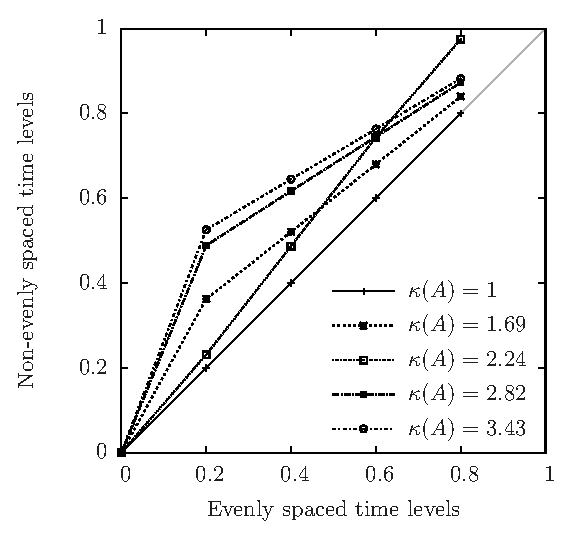
\includegraphics[width=.45\textwidth]{CANAL2_RESIDUAL_VS_CONDITIONNING_TLV_REPARTITION_F2.eps}}
  \caption{Distribution of the time levels on each frequency periods.}
  \label{fig:canal2_distribution_tlv}
\end{figure}
The results in Fig.~\ref{fig:canal_residual_vs_conditionning} show that
for a condition number $\kappa (A) \geq 3.43$ and wave input amplitude
$A_1 = 0.05$, the computation diverges. However, the computations with
the same condition numbers but a smaller input amplitude $A_1 = 0.01$
converge. In fact, the condition number amplifies the errors made
during the iterative process. When the input waves have a smaller
amplitude, the iterative errors are slighter, hence the convergence as
explained \S~\ref{sec:condition_number}.
\begin{figure}[htb]
  \centering \subfigure[$A_1 =
  0.01$]{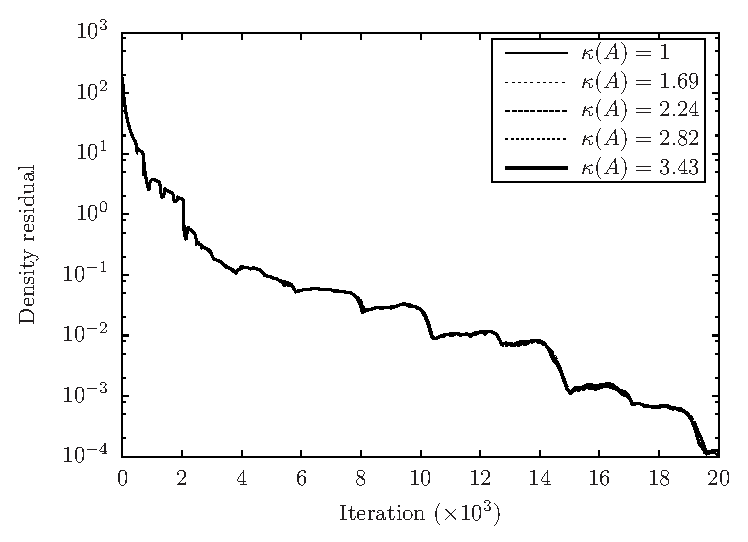
\includegraphics[width=.45\textwidth]{CANAL2_RESIDUAL_VS_CONDITIONNING_AMP001.eps}}
  \quad
  \subfigure[$A_1=0.05$]{\includegraphics[width=.45\textwidth]{CANAL2_RESIDUAL_VS_CONDITIONNING_AMP005.eps}}
  \caption{Relation between the condition number $\kappa (A)$ and the
    convergence of the solution.}
  \label{fig:canal_residual_vs_conditionning}
\end{figure}


\subsection{Validation of the multi-frequency HB method}

To validate the proposed HB method, two non-harmonically related
frequencies are chosen as input for the outlet boundary condition:
$f_1 = 3$~Hz and $f_2 = 17$~Hz.

A classical time-marching scheme is taken for comparison, namely the
Dual Time Stepping scheme (DTS~\cite{Jameson1991}).  The DTS method is
a 2\textsuperscript{nd}-order implicit time-marching scheme.
Convergence in time discretization is obtained after 20~periods using
160~instants per almost-period. Since the frequencies are integers and
coprime, the period is $T=1$~s.  Iterative convergence for the
inner loop is considered achieved when the normalized residuals drop
by $10^{-2}$ within a maximum of 50~sub-iterations.

The results obtained with the DTS scheme are compared to the HB
results for pressure waves amplitudes of $A = A_1 = A_2 = 0.001$.  The
transient of the DTS computation is shown
Fig.~\ref{fig:canal2_transient}, illustrating the wave propagation
with a slight attenuation of the high-frequency waves.
%The waves propagating upstream vanishing with the effect of viscosity
%are highlighted.
\begin{figure}[htbp]
  \centering
  \includegraphics*[width=.7\linewidth]{CANAL2_TRANSIENT.eps}
  \caption{DTS computation: transient propagation of the pressure waves.}
  \label{fig:canal2_transient}
\end{figure}


%Firstly, the DTS results are verified to yield a
%time-converged solution. =>deja dit plus haut !
The results are analyzed for frequencies $1<f< 40~\textrm{Hz}$ and the
dominant frequencies (the one that have the highest amplitudes) are
set for the HB computation.  To do so, pressure signals are probed
upstream, in the middle and downstream of the channel at
$x=[25~\textrm{m}, 50~\textrm{m}, 75~\textrm{m}]$ and $z=0.5$~m
respectively.  The spectrum of the aforementioned unsteady pressure
signals, obtained with a Fourier Transform, are plotted
Fig.~\ref{fig:canal2_dts_fft}.  The labeled frequencies are the
dominant ones, as for each probe, these have a high amplitude. They
are thus selected for the HB computation.  For such frequencies, the
OPT algorithm gives a set of time levels leading to a condition number
of~1.4.
\begin{figure}[htb]
  \centering
  \includegraphics*[width=.6\linewidth]{CANAL2_PROBE_POSITION.eps}

  \vspace{1em}

  \includegraphics*[width=.6\linewidth]{CANAL2_DTS_FFT.eps}
  \caption{Spectrum of pressure signals.}
  \label{fig:canal2_dts_fft}
\end{figure}

A Discrete Fourier Transform is computed at several axis positions,
resulting in the spatial evolution of the different harmonics, which
is used for the comparison of the HB and DTS approaches, in the middle
of the canal ($z = 0.5$~m).  In
Fig.~\ref{fig:canal2_validation_hbt_gear_amp_vs_axis}, the results are
plotted for the frequencies that have been set for the HB computation.
The overall agreement is fair.  Some local discrepancies can be
observed upstream for frequencies $f_2 + 3f_1$, $f_2 - f_1$ and $f_2 -
2f_1$. These are caused by aliasing
 but they are minimal regarding the temporal evolution, as
shown in Fig.~\ref{fig:canal2_validation_hbt_gear_time_ev}, where the
time evolution of pressure signals is extracted at all probes.  The
difference between the HB and the DTS method is negligible, proving
that the proposed HB method is able to reproduce the unsteady
almost-periodic phenomena.
\begin{figure}[htbp]
  \centering
  \includegraphics*[width=.7\linewidth]{CANAL2_VALIDATION_HBT_GEAR_AMP_VS_AXIS.eps}
  \caption{Spatial evolution of the amplitude of the dominant
    frequencies in the channel, for $f_1 = 3$~Hz and $f_2 = 17$~Hz.}
  \label{fig:canal2_validation_hbt_gear_amp_vs_axis}
\end{figure}

\begin{figure}[htb]
  \centering 
  \subfigure[Probe
  1]{\includegraphics[width=.45\textwidth]{CANAL2_VALIDATION_HBT_GEAR_TIME_EV_PROBE_1.eps}}
   \quad\subfigure[Probe
   2]{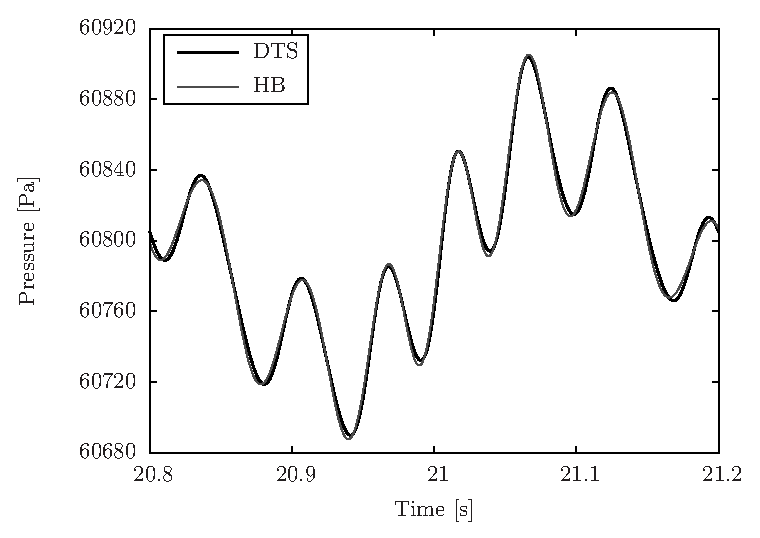
\includegraphics[width=.45\textwidth]{CANAL2_VALIDATION_HBT_GEAR_TIME_EV_PROBE_2.eps}}
   \subfigure[Probe
   3]{\includegraphics[width=.45\textwidth]{CANAL2_VALIDATION_HBT_GEAR_TIME_EV_PROBE_3.eps}}
  \caption{Unsteady pressure signals at different axial positions.}
  \label{fig:canal2_validation_hbt_gear_time_ev}
\end{figure}

The goal of this section was not to show significant CPU savings but
rather the capacity of the present HB method to capture an
almost-periodic flow on a model problem.  It is now applied to a more
complex configuration, namely a turbomachinery element, where its
computational efficiency is also emphasized.






\section{Convection equation solver}




% chapter validation (end)
%     * Advantages
%         - capturing a sinusoidal flow
%         - capturing a wake / clocking effects
%!TEX root = ../main.tex
\section{Advantages} % (fold)
\label{sec:advantages}

\subsection{Capturing a sinusoidal flow} % (fold)
\label{sub:capturing_a_sinusoidal_flow}

Harmonic balance approaches have been developed to
efficiently capture unsteady periodic signals.
In order to set these ideas on a simple example,
let us take the case of an injected signal composed
of the sum of two sine functions: 
\begin{equation}
	u_0(t) = \sin (2 \pi f_1 t) + \sin(2 \pi f_2 t).
\end{equation}




\subsubsection{case 1: $f_1 = f_2 = 1 \text{Hz}$}

This signal is made of a single frequency $f_1 = f_2 = 1 \text{Hz}$.
The mono-frequential harmonic balance computation ran with only one harmonic
is shown Fig.~\ref{fig:convection_sin_1_tsm_n_1}.
\begin{figure}[htbp]
  \begin{center}
    \includegraphics[width=.5\textwidth]{CONVECTION/FIGS/CONVECTION_SIN_1_TSM_N1.pdf}
  \end{center}
  \caption{Convection of a sinusoidal function. Harmonic balance computation
  ran with $f_1$ frequency compared to analytical result}
  \label{fig:convection_sin_1_tsm_n_1}
\end{figure}
The harmonic balance results match perfectly the analytical solution.
This was expected as harmonic balance methods have been developed to
easily capture periodic signals. When these are made of only one frequency,
one harmonic is sufficient to capture all the unsteadiness.

\subsubsection{$f_1 = 1 \text{Hz}$, $f_2 = 2 \text{Hz}$}

A sinusoidal function with a frequency $f_2 = 2f_1$ is now injected.
Two computations are ran. The first has 

\begin{figure}[htbp]
  \begin{center}
    \includegraphics[width=.5\textwidth]{CONVECTION/FIGS/CONVECTION_SIN_2_TSM_N1.pdf}
  \end{center}
  \caption{Convection of a sinusoidal function. Harmonic balance computation
  ran with frequency compared to analytical result}
  \label{fig:convection_sin_2_tsm_n_1}
\end{figure}

\begin{figure}[htbp]
  \begin{center}
    \includegraphics[width=.5\textwidth]{CONVECTION/FIGS/CONVECTION_SIN_2_TSM_N2.pdf}
  \end{center}
  \caption{Convection of a sinusoidal function.}
  \label{fig:convection_sin_2_tsm_n_2}
\end{figure}

\subsubsection{$f_1 = 1 \text{Hz}$, $f_2 = 10 \text{Hz}$}




\underline{What we have learned:} 
\begin{itemize}
  \item from case 1: For a sinusoidal temporal function made of only one frequency,
        only one frequency is needed to capture the field. This is much more efficient
        than a classical time-marching scheme.
\end{itemize}



% subsection capturing_a_sinusoidal_flow (end)

% section advantages (end)
%     * Drawbacks
%         - non evenly spaced timelevels
%         - signal to capture (wake / sinus / step function)
% 
% # Improving the method
%     * algorithm to automatically choose the timelevels
\input{./CHAPTERS/algo_opt}
%     * convergence of spectral methods : analyzing the spectrum of the wake
%     * partial conclusion: we may go to industrial applications
% 
% # application to the aeroelasticity of contra-rotating open rotors
%     * validation of the proposed approach (STCF 11)
%!TEX root = ../../main.tex
\chapter{STCF 11}
\label{stcf11}

\lhead{Chapitre ??. \emph{Chapter Title Here}}

\section{Présentation de la configuration standard 11}
\label{sec:presentation_stcf11}

La configuration standard 11~\cite{Fransson:1999uq}
est une aube de stator de turbine oscillant sur 
son premier mode de flexion à régimes: un subsonique et un
transsonique. Le premier mode est 

\begin{table}[htbp]
  \ra{1.3} \centering
  \begin{tabular}{lccc}
    \toprule
    \phantom{abdefghijk}& $C_t$ & $C_p$ & $\eta$ \\
    \midrule
    Take-off & $-1.448$ & $2.895$ & $0.565$ \\
    Cruise & $-1.067$ & $5.32$ & $0.789$ \\
    \bottomrule
  \end{tabular}
  \caption{Point de fonctionnement.}
  \label{tab:flight_condition}
\end{table} 

\begin{itemize}
  \item un régime subsonique où l'écoulement
        ne présente pas de phénomènes physiques majeurs.
        Ce cas permet de facilement valider le code numérique
        avant de l'éprouver sur un point de fonctionnement plus
        complexe,
  \item un régime transsonique qui se distingue par la 
        présence d'un 
        choc à environ $75\%$ de la corde axiale,
        et d'un bulbe de décollement à $\approx 30\%$
        de la corde axiale.
        Ce cas permet, quant à lui, d'évaluer la robustesse
        du code dans le cas d'un écoulement complexe.
\end{itemize}

La cascade d'aubes est placée dans un canal annulaire fixe de l'École
Polytechnique Fédérale Lausanne~Fig.\ref{fig:canal_annulaire}.
Ce dernier permet d'obtenir un écoulement tant transsonique que subsonique
grâce à la forme de sa veine d'essai. De plus, le canal étant fixe,
l'instrumentation des pales est relativement aisée.
La vibration des pales est assurée par un actuateur électromagnétique
permettant la mise en place d'une onde tournante de type mode à diamètre.

\begin{figure}[htbp]
  \centering
  \includegraphics*[width=0.40\textwidth]{./ANNULAR_CHANNEL.pdf}
  \caption{Canal annulaire}
  \label{fig:canal_annulaire}
\end{figure}


\section{Instrumentation de l'aube}

L'instrumentation est réalisée sur la peau d'une des aubes.
Des sondes de pressions statiques non intrusives permettent
de mesurer la répartition de cette dernière 
le long de la corde axiale. Étant donné le caractère instationnaire
des phénomènes aéroélastiques, l'acquisition temporelle de la pression
statique est réalisée afin de donner les résultats sous forme de partie imaginaire
et réelle du premier harmonique de pression.

Pour la mise en valeur des effets stationnaires, le nombre de Mach isentropique est 
calculé à partir des mesures de pression statique. Ce dernier est défini par
% 
\begin{equation}
  M_{is} = \sqrt{\left[\left(\frac{P_{i0}}{P_s}\right)^{\frac{\gamma - 1}{\gamma}} - 1 \right] \cdot \frac{2}{\gamma -1}},
  \label{eq:mach_isentropique}
\end{equation}
% 
où $P_{i0}$ est la pression totale de référence et $P_s$ la pression statique
mesurée sur la peau de l'aube. Cette dernière évolue le long de la corde axiale.
Étant donné que $P_{i0}$ est constant, le nombre de Mach isentropique va suivre une
évolution similaire à l'inverse de la pression statique, ainsi il peut être
décrit comme l'interprétation de la pression statique sous forme de vitesse
adimensionnée, lorsque la pression totale n'est pas facilement accessible. En effet,
les aubes sont facilement instrumentées par des capteurs de pression statique, car ils 
ne nécessitent pas d'être intrusifs. Ceci est lié à la conservation de la
pression statique ($\frac{\partial P}{\partial n} = 0$ sous hypothèses de Prandtl). En revanche,
les prises de pression totale nécessitent de créer un arrêt isentropique, ce qui 
entraînerait la mise en place de sondes intrusives et de surcroît hors de la surface de
la peau de la pale.

Pour l'évaluation des effets aéroélastiques, des mesures de l'amplitude $\widetilde{Cp}$ et de la
phase $\widetilde{\phi}$ du premier harmonique de pression sont données sous forme de répartition
le long de la corde du profil définies par
% 
\begin{equation}
  \begin{split}
    C_{p, inst} &= \frac{c \cdot \widetilde{P_s}(x)}{h \cdot (P_{i0} - P_{s0})}, \\
    \widetilde{Cp} &= |C_{p, inst}|, \\
    \widetilde{\phi} &= \textrm{arg}(C_{p, inst}),
  \end{split}
  \label{eq:cp_inst}
\end{equation}
% 
où $\widetilde{P_s}(x)$ est l'évolution sur la corde du premier harmonique de pression
et $P_{s0}$ est la pression statique en entrée du canal.

La géométrie, les résultats expérimentaux et les articles associés à la 
configuration standard $11$ sont disponibles sur internet~\cite{STCF11_url}.
Des études sont présentes dans la littérature, principalement pour le cas 
transsonique de par la complexité de l'écoulement qui s'y développe 
\cite{Cinnella:2004fk, Sbardella:2001fk, Duta:2002uq, Campobasso:2003fk}.
Ces derniers montre l'adéquation des résultats numériques avec ceux expérimentaux, 
ce qui en fait un cas test intéressant.

\section{Paramètres numériques}

Le calcul est réalisé avec le code de calcul \textit{elsA}. Un schéma décentré de type
Roe du troisième ordre est choisi. Pour la modélisation de la turbulence, 
le modèle de Spalart-Allmaras est utilisé. Afin de pouvoir comparer les résultats obtenus
avec une approche de référence, les calculs instationnaires sont réalisés avec l'approche
classique dite de pas de temps dual.

L'aube de turbine est maillée en suivant une topologie O4H. Le nombre de points est de 160
autour de l'aube et les $y^+$ calculés sont $\mathcal{O}(1)$, ce qui correspond à l'état de 
l'art pour un tel calcul.

\section{Résultats stationnaires}

\subsection{cas subsonique}

Le cas subsonique est représentatif d'une turbine fonctionnant au point nominal.
L'écoulement ne présente pas de phénomènes particuliers~Fig.~\ref{fig:stcf11_rans_2D_subsonic}.
La répartition de nombre de Mach isentropique est 

\begin{figure}[htbp]
  \centering
  \includegraphics*[width=0.45\textwidth]{STCF11_SUBSONIC_FIELD_MIS_BW.png}
  \caption{Champ stationnaire}
  \label{fig:stcf11_rans_2D_subsonic}
\end{figure}

\begin{figure}[htbp]
  \centering
  \includegraphics*[width=0.45\textwidth]{STCF11_RANS_SUBSONIC.pdf}
  \caption{Répartition du nombre de Mach isentropique fonction de la corde axiale}
  \label{fig:stcf11_rans_mis_subsonic}
\end{figure}



\subsection{cas transsonique}

\begin{figure}[htbp]
  \centering
  \includegraphics*[width=0.45\textwidth]{STCF11_TRANSONIC_FIELD_MIS_BW.png}
  \caption{Champ stationnaire}
  \label{fig:stcf11_rans_2D_transonic}
\end{figure}

\section{Résultats instationaires}

\subsection{cas subsonique}

\subsection{cas transsonique}



% 
% Pour les simulations numériques, 
% 
% Les paramètres numériques utilisés pour les simulations suivantes sont rappelés ci-dessous:
% \begin{itemize}
%   \item schéma spatial de Roe d'ordre 3,
%   \item modèle de turbulence de type $k-l$ de Smith.
% \end{itemize}
% 
% \paragraph{Cartographie de champ 2D}
% 
% Les cartographies de champ 2D sont donnés en figure \ref{fig:stcf11_rans_2D}. La pression statique est représentée en contours et les lignes de courant en traits fins, ou en d'autres termes, la trajectoire que suit le fluide. Le cas subsonique ,\fig \ref{fig:stcf11_rans_2D_subsonic}, ne présente pas de singularité, le fluide accélère sur l'extrados et décélère sur l'intrados de la pale. En revanche, le cas transsonique présente de fortes singularités qui expliquent son étude à des fins de validation. En effet, ce dernier présente deux phénomènes aérodynamiques complexes repérés dans la figure \ref{fig:stcf11_rans_2D_transonic}. 
% \begin{itemize}
%   \item \textit{zone I}: bulle de décrochage. Avant que le profil décroche (c'est à dire que les lignes de courant ne suivent plus le profil), une bulle de décrochage peut se former. Or cette non-linéarité va réagir avec les vibrations de la pale comme nous le verrons plus tard.
%   \item \textit{zone II}: cette zone présente un choc. C'est un phénomène dimensionnant dans une turbomachine. On peut le visualiser par la discontinuité en pression qu'il présente.
% \end{itemize}
% 
% 
% \paragraph{Comparaison avec les résultats expérimentaux}
% Comme rappelé dans la section \ref{sec:presentation_stcf11}, des résultats stationnaires expérimentaux sont donnés sur le site internet du KTH. La comparaison avec les présents résultats est reportée en figure \ref{fig:stcf11_rans_expe}.
% 
% Ces résultats montrent la bonne adéquation entre l'expérience et les calculs numériques. Les principales disparités observées sont similaires à celle rencontrées dans la littérature:
% \begin{itemize}
%     \item cas subsonique: surestimation du Mach isentropique sur l'extrados de la configuration lors de la recompression,
%     \item cas transsonique: sous estimation de l'intensité du choc sur l'extrados et surestimation de la position du choc (zone II détaillé précédemment), même si les disparités dans les mesures expérimentales mettent en avant leurs incertitudes.
% \end{itemize}
% 
% 
% 
% \begin{figure}[H]
%     \center
%     \subfigure[cas subsonique]{ 
%       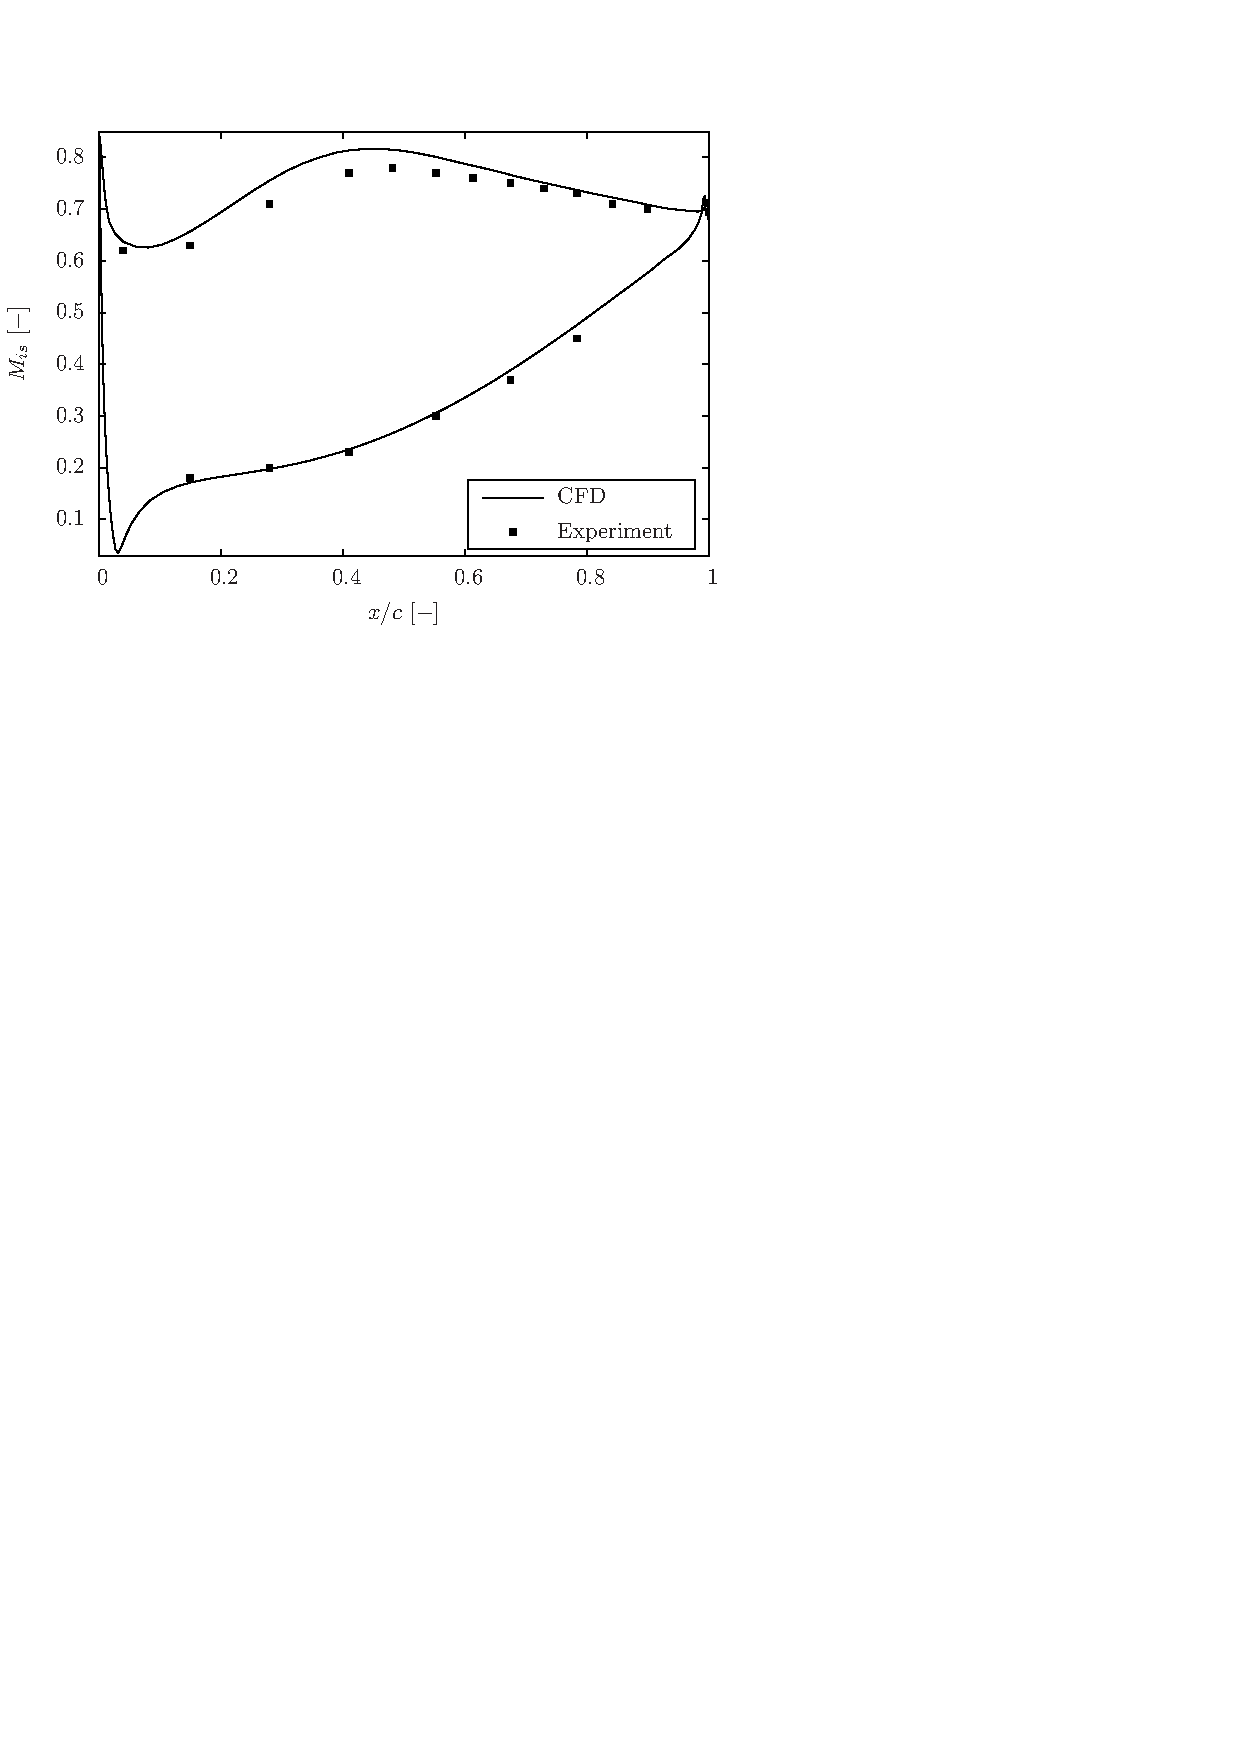
\includegraphics[width=7.5cm]{IMAGES/STCF11_RANS_SUBSONIC.pdf}}
%     \subfigure[cas transsonique]{ 
%       \includegraphics[width=7.5cm]{IMAGES/STCF11_RANS_TRANSONIC.pdf}}
%     \caption{Résultats stationnaires}
%     \label{fig:stcf11_rans_expe}
% \end{figure}
% 
% \section{Résultats aéroélastiques}
% 
% Des premiers résultats aéroélastiques ont été obtenus avec le code de calcul \elsa. La fréquence du mode imposé est $211.6 Hz$ et l'amplitude de $0.0035$.
% Les résultats sont donnés en terme d'évolution de l'amplitude et de la phase du premier harmonique de pression sur la pale. La figure \ref{fig:stcf11_ael} montre les résultats obtenus avec \elsa avec une approche DTS et HBT. Les résultats sont comparés à l'expérience et aux résultats de Cinnella et al. (voir Réf. \cite{Cinnella:2004fk}). En effet, les résultats numériques obtenus par ces derniers sont téléchargeables sur internet \footnote{http://cemec.poliba.it/BENCHMARK\_SC11.txt}, ce qui permet une comparaison supplémentaire.
% 
% L'analyse de ces résultats permet de dire que:
% \begin{itemize}
%   \item la prédiction des paramètres conditionnant l'amortissement est bonne que ce soit en DTS ou en HBT. Rien ne permet de qualifier l'une ou l'autre de meilleure. Ainsi, l'approche HBT pour prédire le flottement est validée,
%   \item les régions qui "pulsent" (comprendre où l'amplitude du coefficient de pression augmente) semble être les régions où il y a des phénomènes physiques importants. En effet, la région du bulbe de décrochage ($0 \leq x/c \leq 0.3$, zone I présentée dans la partie précédente) et la région du choc ($0.7 \leq x/c \leq 0.9$, zone II) ont toutes les deux un pic de coefficient de pression.
% \end{itemize}
% 
% 


% Fransson et al.:
% 
% - veine annulaire non tournante cascade de EPF-Lausanne
% - 20 pales excitée électromagnitiquement et contrôller pour vibrer en mode tournant
% - les suspensions des pales sont contruites afin de reproduire la fréquence propre
% et la direction du mode de flexion de la pale entrain de faire un movement rigide
% - STCF 11: choc droit à 75\% de la pale sur l'extrados
% - différences dans l'amortissement du à de petites différences dans la région du choc
% - mesures de pression totale et statique dans les plans e1 et e2 ainsi que derrière la cascade
% - les mesure pariétales sont faites au moyen de "pressure-taps" pour le cas stationnaires et de
% "miniaturized piezo-resistive pressure transducer" pour le cas instationnaire, embarqué à mi-hauteur de pale,
% sur différentes pales
% - en changeant un peu les conditions, le choc peut varier de 5\% en position
% - raisons de variations entre les expé et le numérique: effets du fluide réel non
% capté par les méthodes numérique ou perdu à cause des techniques de mesure (effet 3D, 
% couche limite des murs (hub/shroud), erreurs sur les relevés de pression, estimation des angles 
% du fluide, moyennage des grandeurs en azimuth et en hauteur radial)
% - amortissement varie énormement en fonction des conditions amonts
% dans le cas transsonique (fig 4.)
% - en revanche on a des tendances dans les mesures locales 
% - c'est la position du choc qui est la première source d'incertitude

% Cinnella et al.:
% 
% - pour les différents IBPA, elle multiplie le nb de canaux:
% np=z*360deg/IBPA, où z est l'entier minimum qui donne une valeur
% entière de np
% - présentation du cas STCF 11: conditions d'entrée (Mach et angle de l'écoulement)
% et reynolds de 1,2.10+6 basé sur la longueur de la corde et les conditions amonts
% - remise en cause de l'expé lorsque les bars de confiance à 95 \% sont de l'ordre
% de la valeur moyenne du point, gros écart lorsque Fransson et al. modifient les
% conditions amonts -> on regarde les résultats locaux

% Campobasso et Giles:
% 
% - ils font du LUR, couplage faible avec une méthode GMRES pour stabiliser
% les oscillations qu'ils obtiennent dans les champs stationnaires.
% - en fait ces oscillations sont dues à la physique du pb (décollement,
% vortex shedding ...)
% - ils imposent l'IBPA comme un déphasage complexe (comme nous)
% - ils calculent le travail du fluide sur la structure (donc pas les
% courbes d'amortissement de Fransson directement)

% Duta et al.:
% 
% - belle intro sur l'utilité de l'aéroélasticité
% - biblio sur méthodes de couplage faible
% - place du LUR dans simu aéroélastiques
% - LUR: hypothèse périodicité et petites perturbations
% - calcul adjoint pour estimer la réponse forcée de différents
% type de distortions amonts
% - si le sillage impacte la pale de manière uniforme, la réponse forcée sera maximale,
% si on a un déphasage du moment de l'impacte: déphasage=> minimisation
% du travail du fluide sur la structure

% Sbardella et Imregun
% 
% - papier de ref sur l'AEL
% - calculs 3D AEL bien mais les designers ont besoin de calculs qui tournent vite
% - le flottement est généralement un phénomène qui apparait dans des conditions off-design
% - sur prédiction sur le cas subsonique à mi-corde, mais raison de cet effet
% discuter dans Fransson et al.
% - nombre de Mach pré-choc est très sensible aux conditions d'entrée pour le 
% cas transsonique (fransson et al.), d'où les différences avec les essais
% - il vaut mieux que la turbulence ne soit pas gelée
% - rapport 30 sur le temps de calcul

% Fransson: Annular cascade experiments
% 
% - avantages de la veine d'essai annulaire non tournante:
%       * pas de murs latéral dans la direction circonférentielle => pas de réflexion des ondes de pression
%       * écoulement périodique dans le domaine
%       * instrumentation facile car pas de rotation
%       * écoulement supersonic possible grâce à la forme du tube d'écoulement
% - peut accueillir 20 pales
% - les pales sont en vibration forcée par le biais d'un exciteur électromagnétique
% la vibration des pales est mesurée par des capteurs de déplacement inductifs.
% ces capteurs sont fixés sur un anneau d'impact. Ce dernier est controllé axialement
% par un système hydraulique. Cela permet de limiter la vibration des pales si elles 
% commencent à osciller en flottement naturel (auto-déclanché) afin de ne pas casser
% les amortisseurs. Un système électronique de contrôle permet d'établir et de maintenir un 
% mode de vibration organisé de la cascade.
% - les frequences d'excitations doivent être proches de la fréquence propre 
% du système pale-mass-ressort
%     * aeroelasticity of an isolated contra-rotating open rotor
%     * aeroelasticity of an installed contra-rotating open rotor


%----------------------------------------------------------------------------------------
%	THESIS CONTENT - APPENDICES
%----------------------------------------------------------------------------------------

\addtocontents{toc}{\vspace{2em}} % Add a gap in the Contents, for aesthetics

\appendix % Cue to tell LaTeX that the following 'chapters' are Appendices

% Include the appendices of the thesis as separate files from the Appendices folder
% Uncomment the lines as you write the Appendices

%!TEX root = ../main.tex
\chapter{Validation of the convection code}
\label{Appendix_convection_code}

%\input{./Appendices/AppendixB}
%\input{./Appendices/AppendixC}

\addtocontents{toc}{\vspace{2em}} % Add a gap in the Contents, for aesthetics

\backmatter

%----------------------------------------------------------------------------------------
%	BIBLIOGRAPHY
%----------------------------------------------------------------------------------------

\label{Bibliography}

\lhead{\emph{Bibliography}} % Change the page header to say "Bibliography"

\bibliographystyle{unsrtnat} % Use the "unsrtnat" BibTeX style for formatting the Bibliography

\bibliography{biblio} % The references (bibliography) information are stored in the file named "Bibliography.bib"

\end{document}  